%______________________________________________
%             CPT6123 ASSIGNMENT 2
% ______________________________________________

\documentclass[a4paper, 12pt]{article}
\usepackage[T1]{fontenc}
\usepackage[utf8]{inputenc}
\usepackage{apacite}
\usepackage{mathptmx}
\usepackage{enumerate}
\usepackage[margin=1.0in]{geometry}
\usepackage{xspace}
\usepackage{graphicx} % Required for inserting images
\usepackage{multirow}
\usepackage{adjustbox} 
\usepackage{array}
\usepackage{tikz}
\usetikzlibrary{positioning,shapes.geometric}
\usepackage[dvipsnames]{xcolor}
\usepackage{url}
\usepackage{hyperref}
\graphicspath{{Images/}}

\renewcommand{\baselinestretch}{1.5}

\newcommand\nd{\textsuperscript{nd}\xspace}
\newcommand\rd{\textsuperscript{rd}\xspace}
\newcommand\nth{\textsuperscript{th}\xspace} %\th is taken already

\setlength\parindent{0pt} % set paragraph indent to zero

%______________________________________________
%                 GROUP 8 TT9L
% _____________________________________________

\author{
Amany Sharaf El Deen Sami Al Horani \quad 1221305230 \quad 25\%\ \\
Thirissha Gangatharan \quad 1211106376 \quad 25\%\ \\
Jaroon, Nasreen Hussein Moqbel \quad 1211105750 \quad 25\%\ \\
Chin Yee Chung \quad 1211111435 \quad 25\%\ \\\\
}
\title{ Ethical Challenges in \\
AI-Driven Healthcare: A Data Science Perspective
  }
  

\begin{document}
\maketitle

\section*{Executive Summary}
This research explores the ethical challenges in AI-driven healthcare, highlighting concerns such as algorithmic bias, data privacy issues, and the lack of transparency in AI-driven systems. The primary objective of this study is to identify and analyze the primary ethical challenges associated with the implementation of AI-driven healthcare systems, focusing on algorithmic bias, transparency, and data privacy. The research employs a mixed-methods approach, combining quantitative and qualitative techniques, including a comprehensive literature review, surveys, interviews, and case studies. The expected result of this study is to enhance the understanding of ethical issues in AI-driven healthcare, especially within intelligent health information systems. By bridging the gap between AI ethics principles and their practical application, the research aims to contribute actionable strategies to enhance the ethical deployment of AI in healthcare.
\hfill
\\\\
\textbf{Keywords:} AI ethics, healthcare, algorithmic bias, data privacy, transparency \\

\pagebreak
\tableofcontents
\pagebreak
% ______________________________________________
%                  INTRODUCTION
% ______________________________________________

\section{Introduction} 
Artificial intelligence (AI) is transforming the way doctors and hospitals operate by quickly analyzing and interpreting vast amounts of medical information. It assists with tasks such as managing paperwork and identifying critical details about patient care. One significant area where AI is making an impact is in intelligent computer systems that analyze large datasets to help doctors diagnose potential issues and determine the most effective treatments \cite{Gujral2020}. While AI is expected to enhance efficiency and improve patient outcomes, there are also significant concerns to consider, such as safeguarding personal information, ensuring fairness in technology, and maintaining patient understanding of their care processes \cite{Fatima2024}.\\

AI is significantly enhancing doctors' ability to diagnose eye disorders more effectively than before. It employs specific techniques to detect conditions such as diabetic retinopathy, glaucoma, and age-related diseases \cite{Fatima2024}. However, before we can fully integrate AI into hospitals and clinics, it is essential to address several critical limitations. We must ensure that AI operates fairly, avoids errors based on inaccurate data, and that we comprehend its decision-making processes, particularly concerning patient care. This study examines how AI can assist in diagnosing eye disorders while also considering the crucial ethical guidelines that must be followed as its use expands in healthcare \cite{Sarker2021}.\\

As healthcare providers adopt new technologies, it is critical to establish clear regulations for their use, particularly in the case of artificial intelligence (AI). This research will investigate the potential of AI, as well as the ethical challenges it presents, offering insights into how AI can enhance healthcare delivery while protecting patient rights and ensuring equitable access to these new technologies \cite{Nassar2021}. Its aim is to ensure that all individuals have fair access to these advancements and that patients are treated safely and justly. This introduction lays the groundwork for a more in-depth examination of how AI can assist in medicine, as well as the essential criteria that must be considered.\\

% ______________________________________________
%                  PROBLEM STATEMEMT
% ______________________________________________

\section{Problem Statement}
The integration of AI and data science in healthcare, particularly in the development of intelligent health informatics systems, presents both significant opportunities and ethical challenges. While AI technologies have demonstrated remarkable capabilities in analyzing large datasets, improving diagnostic processes, and enhancing decision-making in healthcare, they also introduce risks related to algorithmic bias, data privacy, and the transparency of AI-driven decisions. These risks are particularly pronounced in applications such as retinal disease diagnosis, where the accuracy of AI models must be weighed against the ethical implications of their deployment in clinical settings. Furthermore, the gap between AI ethics principles and their practical application highlights the necessity of embedding ethical considerations throughout the entire AI system lifecycle.

\section{Justification} The use of AI in healthcare systems presents a double-edged sword, offering unprecedented opportunities for improving patient care while simultaneously posing ethical dilemmas. As AI technologies become more pervasive, understanding their implications becomes crucial for ensuring that advancements do not compromise patient rights or exacerbate existing disparities in healthcare access. This research is justified by the pressing need to explore these ethical challenges comprehensively.\\

The concerns surrounding algorithmic bias, data privacy, and transparency are not merely theoretical; they directly impact patient trust and the efficacy of AI applications in healthcare settings. By identifying and analyzing these issues, this study seeks to establish a framework for ethically deploying AI technologies that prioritize patient welfare and promote equity in healthcare delivery. Additionally, the findings aim to inform policymakers, healthcare providers, and technology developers about best practices in implementing AI systems responsibly, ultimately leading to safer, more effective healthcare solutions. This research fills a critical gap in understanding the intersection of AI, ethics, and healthcare, thereby paving the way for more informed and responsible AI applications in clinical practice.

\section{Research Questions, Hypotheses, and Objectives}
% ______________________________________________
%               RESEARCH QUESTIONS
% ______________________________________________

\textbf{\large 4.1 \hspace{5mm} Research Questions}
\begin{itemize}
\item What are the primary ethical challenges in implementing AI-driven healthcare systems from a data science perspective?

\item How effective are current ethical frameworks in addressing the practical challenges of AI implementation in healthcare?

\item What strategies can be developed to bridge the gap between AI ethics principles and their practical application in healthcare data science?
\end{itemize}

% ______________________________________________
%                  HYPOTHESES
% ______________________________________________

\textbf{\large \\4.2 \hspace{5mm} Hypotheses}
\begin{itemize}
\item If complete ethical frameworks are implemented in the use of AI and big data analytics for decision-making, then they will help decrease ethical problems such as algorithmic bias, lack of transparency, accountability, and data privacy and security, thereby improving the ethical application of these technologies. 

\item If advanced analytics methods, including machine learning modeling, are applied to data-driven applications, then they will significantly improve the intelligence and capabilities of these applications across various real-world fields, such as business, healthcare, and cybersecurity, leading to more effective smart decision-making. 

\item If ChatGPT is utilized into data science workflows, then it will increase the output by automating tasks such as data cleaning, model training, and result interpretation, while providing new information from unstructured data. 

\item If AI-driven retina disease detection systems are utilized in clinical practice with attention to ethical considerations such as patient privacy, informed consent, and algorithmic bias, then they will improve the diagnostic accuracy, early detection, and patient care outcomes, while addressing challenges related to scalability, the validity in general, and professional responsibility.
\end{itemize}
\pagebreak
% ______________________________________________
%                   OBJECTIVES
% ______________________________________________

\textbf{\large 4.3 \hspace{5mm} Objectives}
\begin{itemize}
\item To identify and understand the main ethical challenges that arise when AI-driven healthcare systems are used, particularly focusing on concerns like algorithmic bias, transparency, and protecting patient privacy. 

\item To examine how well current ethical frameworks address these challenges and explore how they can be practically applied in real-world healthcare settings involving data science.

\item To review specific case studies, such as AI-driven retina disease detection, in order to understand the influence of ethical considerations on diagnostic accuracy, early detection, and overall patient care.

\item To create actionable strategies that can close the gap between AI ethics principles and their practical use in healthcare, with an emphasis on transparency, accountability, and patient-centred care.
\end{itemize}

This research aims to contribute to the ongoing discussions on the ethical use of AI in healthcare, offering insights into how these technologies can be responsibly developed and implemented to maximize benefits while reducing potential risks.
\pagebreak
% ______________________________________________
%                LITERATURE REVIEW
% ______________________________________________

\section{Literature Review}
\subsection{Data Science and Analytics: An Overview from Data-Driven Smart Computing,  Decision-Making, and Applications Perspective (Iqbal H. Sarker, 2021)}
This paper provides a comprehensive overview of data science and advanced analytics in the context of the Fourth Industrial Revolution (Industry 4.0). It emphasizes the importance of extracting knowledge from various types of data, such as IoT data, business data, and health data, to enable smart decision-making in different application domains. The paper discusses how advanced analytics methods, including machine learning, can enhance the intelligence and capabilities of applications, making the computing process more automatic and smarter. 
\begin{center}
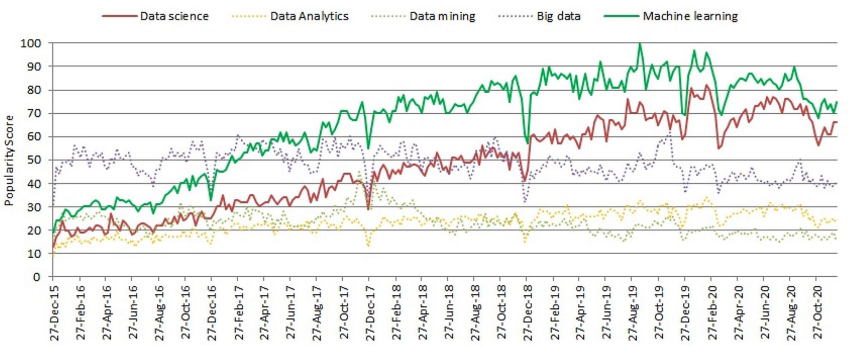
\includegraphics[scale=0.9]{Figure1.png}\\
\small Figure 1: The worldwide popularity score of data science compared with relevant areas in a range of 0 (min) to 100 (max) over time, where x-axis represents the timestamp information and y-axis represents the corresponding score.\normalsize
\end{center}

Figure 1 shows the increasing worldwide popularity of data science and related fields, such as data analytics, data mining, big data, and machine learning, over the last five years. The data, sourced from Google Trends, highlights the growing interest and relevance of these domains in the digital age.\\

 The authors highlight ten potential real-world application domains where data-driven smart computing can be applied. These domains include business, healthcare, cybersecurity, and urban data science, among others. The paper also delves into various advanced analytics methods, such as regression analysis, classification, clustering, and deep learning, explaining their principles and applicability in real-world scenarios. The goal is to provide actionable insights and deeper knowledge about data to support intelligent decision-making.\\
 
Finally, the paper addresses the challenges and potential research directions in the field of data science. It aims to serve as a reference point for researchers, decision-makers, and application developers interested in data-driven solutions for real-world problems. By understanding and applying advanced analytics methods, the paper suggests that significant improvements can be made in various application areas, ultimately contributing to the advancement of smart computing and decision-making in the digital age.

\begin{center}
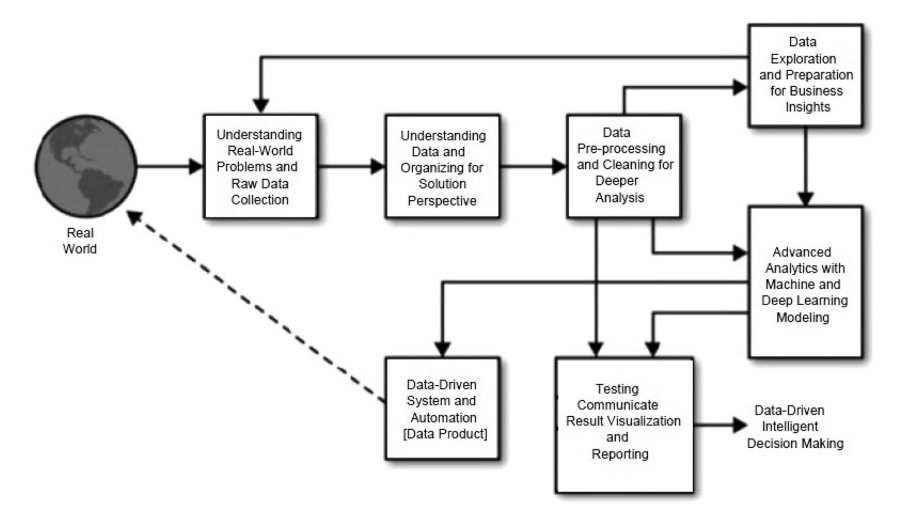
\includegraphics[scale=0.7]{Figure2.png}\\
\small Figure 2: An example of data science modeling from real-world data to a data-driven system and decision making. \normalsize
\end{center}

This figure illustrates the steps involved in data science modeling, starting from understanding business problems to the final stage of data product and automation. It highlights key processes such as data understanding, data preprocessing, machine learning modeling, and evaluation. \\

\textbf{Link to Research Objectives:} This overview discusses the significance of data science in healthcare decision-making, emphasizing advanced analytics methods. This aligns with our first research objective, as it highlights the potential ethical challenges related to algorithmic bias and data privacy in AI-driven systems. Understanding these aspects is important for ensuring ethical applications in healthcare.


\subsection{Ethical Dilemmas in AI-Powered Decision-Making: A Deep Dive into Big Data-Driven Ethical Considerations (Ahmed Nassar & Mostafa Kamal,  2021)}
The article delves into the complex ethical dilemmas posed by AI-powered decision-making, highlighting key issues such as algorithmic bias, transparency, and accountability. These concerns are particularly relevant in critical sectors like healthcare and finance, where the decisions made by AI systems can significantly impact individuals' lives. For instance, biased algorithms can perpetuate unfair outcomes, such as denying people access to healthcare or financial services based on flawed data patterns. The lack of transparency in how these algorithms function exacerbates the problem, as it becomes difficult for affected individuals to understand or challenge decisions that may negatively affect them. Accountability is another pressing issue, as determining responsibility for AI-driven decisions is often unclear, raising questions about liability and governance.\\

Moreover, the integration of big data into AI decision-making introduces additional ethical concerns. The vast amounts of data used to train AI systems often include sensitive personal information, leading to worries about data privacy, security, and informed consent. Without proper ethical guidelines, the misuse of big data can result in violations of individual rights, such as unauthorized surveillance or exploitation of personal data for profit. The article emphasizes the need for ethical frameworks to govern both the collection and use of big data, ensuring that AI systems respect privacy and security while making decisions that affect people’s lives.\\

To navigate these ethical challenges, the article explores several ethical frameworks, including utilitarianism, deontology, and virtue ethics. Utilitarianism, for example, focuses on maximizing overall benefits while minimizing harm, making it a useful approach for evaluating the societal impact of AI technologies. Deontology emphasizes the importance of duty and following ethical principles, regardless of outcomes, while virtue ethics highlights the need to cultivate moral character in individuals developing and deploying AI systems. These frameworks provide valuable perspectives on how to ensure that AI technologies are designed and implemented in ways that align with human values and ethics.\\

In response to these challenges, the article offers several practical recommendations for fostering ethical AI practices. Enhancing transparency in AI algorithms is crucial, allowing users to understand how decisions are made and encouraging trust in AI systems. Addressing algorithmic bias is another key recommendation, as this requires regular auditing and refining of AI models to eliminate unfair or discriminatory outcomes. Promoting ongoing education and awareness about AI’s ethical implications is also essential, both for developers and users of AI systems. Lastly, the article calls for the establishment of industry standards and regulations to provide clear guidelines for ethical AI and big data practices, ensuring that technology is used responsibly across sectors.\\

\textbf{Link to Research Objectives:} This article explores ethical dilemmas in AI decision-making, focusing on issues like algorithmic bias, transparency, and accountability. This directly addresses our first research objective, providing insight into the ethical challenges faced by AI-driven healthcare systems. It sets the stage for examining how current frameworks can address these dilemmas.


\subsection{From AI ethics principles to data science practice: a reflection and a gap analysis based on recent frameworks and practical experience (Llina Georgieva, Tjerk Timan, Claudio Lazo \&\ Anne Fleur van Veenstra, 2022)}
The research investigates the challenges of applying AI ethics from theory to practice within data science. It highlights the growing need to operationalize AI ethics by converting broad ethical principles into practical guidelines that fit seamlessly into the AI development process. By carefully mapping these principles onto different stages of AI service and product development, the study identifies key gaps, particularly in governance, stakeholder engagement, and the practical application of ethics in AI systems.\\

The authors offer a critical review of ethical frameworks proposed by organizations like the European Commission’s High-Level Expert Group on AI (HLEG). While these frameworks mark progress, the research points out a significant gap between theoretical guidelines and their practical use. Data scientists and organizations often struggle to apply these ethical principles due to a lack of clear, actionable guidelines and effective governance models. This gap frequently results in inconsistent ethical practices throughout the AI development lifecycle, especially during crucial stages such as design and testing.\\

Moreover, the research emphasizes the need for comprehensive governance structures that clearly define responsibilities throughout the AI lifecycle. The authors argue that implementing AI ethics effectively requires not just technical solutions but also broader organizational and societal engagement. They highlight that current practices often focus on addressing harm in the later stages of AI deployment, rather than integrating ethical considerations from the outset. This reactive approach, they argue, falls short of the human-centered ideals many ethical frameworks aim to achieve.

\begin{center}
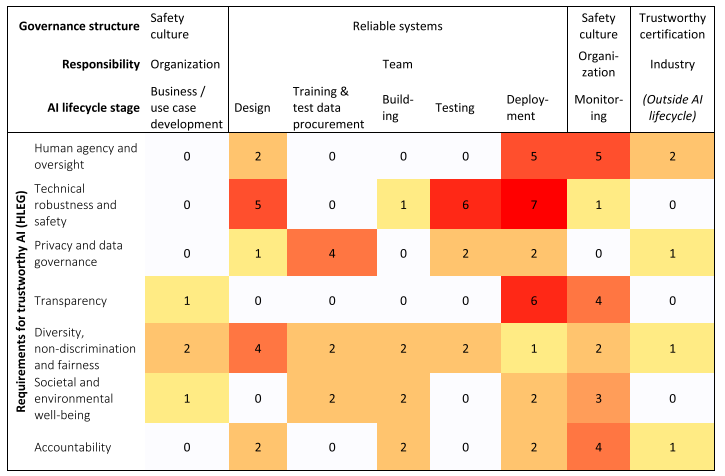
\includegraphics[scale=0.9]{Figure3.png}\\
\small Figure 3: Heatmap of trustworthy AI requirements across the AI lifecycle, and its corresponding governance structures and responsible stakeholders. \normalsize
\end{center}

This heatmap illustrates how ethical principles align with different stages of the AI lifecycle, emphasizing the need for transparency, diversity, and privacy from the business development phase to human oversight in the monitoring phase.\\

The research advocates for a more integrated approach that engages all relevant stakeholders throughout the entire AI lifecycle. This would ensure that ethical principles are not applied in a fragmented way but are systematically incorporated into the development process. By doing so, the study argues for stronger governance models that balance ethical, technical, and political considerations, ultimately leading to the development of more responsible and trustworthy AI systems.\\

\textbf{Link to Research Objectives:} This paper investigates the challenges of applying AI ethics from theory to practice. This is linked to our second research objective, which examines how well current ethical frameworks address the challenges posed by AI in healthcare. By identifying gaps in practical application, this research will inform our understanding of the necessary adaptations for effective implementation.


\subsection{The Role of ChatGPT in Data Science: How AI-Assisted Conversational Interfaces Are Revolutionizing the Field (Hossein Hassani \&\ Emmanuel Sirmal Silva, 2023)}
The research paper discusses the increasing importance of artificial intelligence, specifically the use of ChatGPT, in transforming data science. It talks about the rise of ChatGPT, an AI chatbot platform created by OpenAI, as a key tool in streamlining and improving different parts of data science processes. Nevertheless, the article also points out various difficulties linked to this technology, including biases in AI results, ethical issues, and the risk of plagiarism. The need to balance the advantages of AI with ethical considerations is emphasized in the problem statement to promote responsible utilization.\\

The research relies on a comprehensive method, starting with an in-depth examination of ChatGPT's structure, which includes its core Transformer model and the training procedures that it goes through. The methodology also involves case studies and examples showcasing how ChatGPT can be used to automate data science activities like data cleaning, text classification, and sentiment analysis. Furthermore, the study explores the limitations of ChatGPT by evaluating its effectiveness in comparison to other AI models and investigating its capacity for creating artificial data and assisting in programming assignments.\\

The findings suggest that ChatGPT can greatly improve the effectiveness and precision of data science assignments. It stands out in creating logical and appropriate text within the context, automating tasks, and evaluating unstructured data. Nevertheless, the findings also demonstrate limitations, such as the model depending on extensive data sets for education, which can result in difficulties in settings with limited resources. Moreover, although ChatGPT excels in numerous situations, it can generate unreal or unsuitable replies in complicated or sensitive scenarios.\\

The conversation explores into the balance of benefits and obstacles when including ChatGPT into data science. The writers stress how ChatGPT could widen the access to data science, enabling those with no knowledge to participate in programming and data analysis more easily. Nevertheless, they warn against extreme dependence on AI, highlighting the requirement of human supervision, especially in guaranteeing ethical AI application and reducing biases. The article also emphasizes the importance of continuous training and career advancement to prepare data scientists with the necessary abilities to responsibly use ChatGPT.\\

The paper ends by explaining various potential areas for future research. This involves enhancing ChatGPT's skills in managing complicated data science assignments, boosting its capacity to produce artificial data, and strengthening its collaboration with other AI tools. The writers also propose that upcoming advancements should prioritize on implementing the moral and legal obstacles linked with AI, specifically in guaranteeing that AI-powered technologies are being used in a way that helps society and prevents possible harm. In addition, the article emphasizes the need for further investigation into the lasting effects of AI in data science and the development of regular procedures for its implementation in various applications.\\

\textbf{Link to Research Objectives:} This article discusses how AI-assisted conversational interfaces like ChatGPT are transforming data science, particularly in healthcare. This aligns with our second research objective by examining how existing ethical frameworks can be applied to ensure responsible AI use in healthcare settings. Understanding the implications of conversational AI in medical contexts is essential for addressing ethical challenges related to transparency and patient interaction.


\subsection{Enhancing retinal disease diagnosis through AI: Evaluating performance, ethical considerations, and clinical implementation (Maryam Fatima, Praveen Pachauri, Wasim Akram, Mohd Parvez, Shadab Ahmad \&\ Zeinebou Yahya, 2024)}
This research paper delves into the ethical considerations and challenges associated with the integration of artificial intelligence (AI) in retina disease detection. AI technologies have made notable strides in improving diagnostic accuracy, facilitating early disease detection, and boosting overall efficiency and patient care in ophthalmology. However, the adoption of AI systems necessitates careful attention to ethical issues, including patient privacy, informed consent, algorithmic bias, and professional accountability. It is crucial to tackle these issues to guarantee that AI-driven solutions are deployed in a way that maintains patient safety and fairness.\\

Moreover, it is stated in the research paper that AI technology can aid doctors in treatment planning and monitoring by analyzing longitudinal data to track disease progression and treatment responses as shown in Figure 4. This data aids doctors in making informed decisions, providing personalized care, and enhancing patient outcomes.

\begin{center}
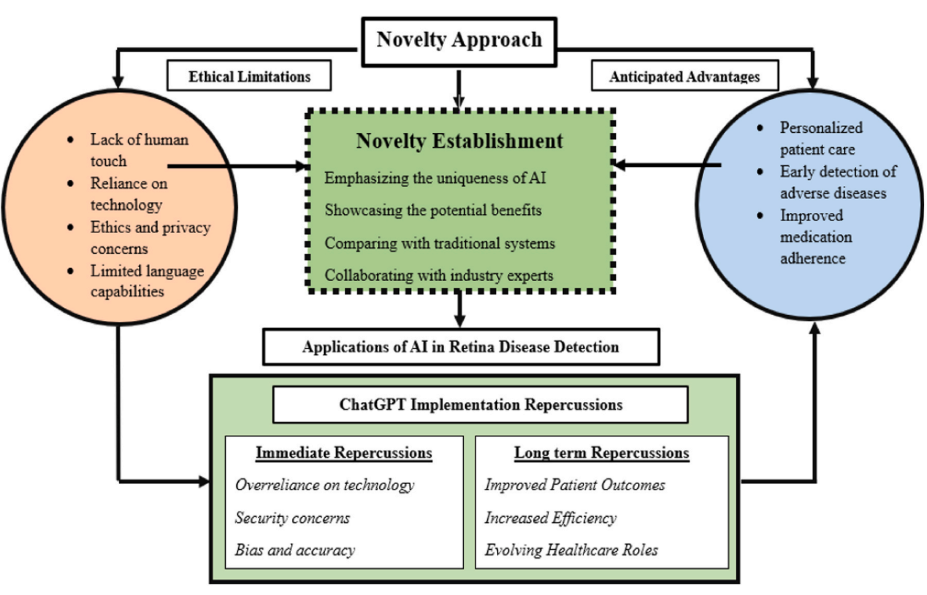
\includegraphics[scale=0.73]{Figure4.png}\\
\small Figure 4: Framework for understanding potential applications of AI in Retina disease detection systems \normalsize
\end{center}

The research methodology employs a thorough approach to assess the effectiveness and ethical implications of AI. It begins with a literature review of existing AI applications in retinal diagnostics, focusing on techniques such as convolutional neural networks (CNNs) and machine learning algorithms used to detect conditions like diabetic retinopathy, age-related macular degeneration, and glaucoma. This is followed by the collection and analysis of retrospective clinical datasets, which provide a basis for assessing the performance of AI algorithms. Various models are developed and tested, with performance evaluated using metrics such as accuracy, sensitivity, specificity, and AUC-ROC. The study also addresses ethical considerations by examining frameworks and guidelines to ensure responsible AI integration.\\

The study's findings emphasize several key outcomes. AI algorithms exhibit high accuracy and sensitivity in detecting retinal diseases, effectively identifying conditions such as diabetic retinopathy, age-related macular degeneration, and glaucoma. Nonetheless, ethical challenges persist, particularly concerning patient privacy, informed consent, and the risk of algorithmic bias. Real-world validation studies confirm the practical utility of AI systems in clinical settings, demonstrating their potential to enhance diagnostic efficiency and patient care. However, the effectiveness of AI algorithms relies on the diversity and representativeness of the training datasets, underscoring the importance of comprehensive and varied data to ensure reliability across diverse patient populations.\\

The discussion underscores the complex balance between the benefits and challenges of AI in retinal diagnostics. Although AI provides significant enhancements in accuracy, early detection, and efficiency, ethical issues such as patient privacy, informed consent, and algorithmic bias must be carefully managed. The study also acknowledges limitations, including biases in datasets, challenges in algorithm interpretability, and the lack of standardized protocols across healthcare institutions. Future research should focus on advancing AI techniques, such as deep learning and the integration of multimodal data to improve diagnostic accuracy and broaden AI capabilities. Integrating AI with wearable devices and telemedicine platforms could improve accessibility and facilitate remote monitoring. Long-term studies are necessary to assess the enduring effects and cost-effectiveness of AI-based diagnostics. Additionally, ongoing efforts to address ethical and regulatory challenges are essential for the responsible and equitable implementation of AI technologies in healthcare.\\

\textbf{Link to Research Objectives:} This study evaluates the use of AI in diagnosing retinal diseases, focusing on both performance metrics and ethical considerations. This supports our third research objective, as it provides specific case studies that highlight the influence of ethical considerations on diagnostic accuracy and patient outcomes. The findings will help us understand how ethical frameworks can enhance the effectiveness of AI in clinical practice.


\subsection{Artificial Intelligence and Data Science for Developing Intelligent Health Informatics Systems (Garima Gujral, Mariappan Muthiah \&\ Shivarama J, 2020)}
In the medical science field, the 21st century has seen a major shift as healthcare organizations are more and more utilizing advanced technologies. One of the most revolutionary advancements is the implementation of Artificial Intelligence (AI), allowing machines to resemble the human cognitive abilities. AI has the capacity to be beneficial in healthcare in many areas such as administrative duties, research, and education. The digital transformation has enabled AI to manage extensive data sets, address complex issues, and improve the examination of huge amounts of data that used to rely on human intelligence. Even with these advancements, issues like having too much information and ineffective information recovery systems continue to exist in healthcare, making AI must be used to improve productivity and quality.\\

The article examines current research and models to understand the influence of AI on the healthcare industry. It talks about the importance of building thorough training databases crucial for advancing AI technology, specifically in the field of medical image acknowledgement. The study highlights the significance of excellent data and investigates the utilization of mobile health (m-Health) devices and apps for collecting and analyzing data. It also explores the creation of AI algorithms, emphasizing the importance of having both labelled and unlabelled data available and including a lot of health data to discover new disease connections. The research covers government efforts and policies in India that influence the use and control of AI in the healthcare sector.\\

The report shows that AI has greatly increased the capacity to handle and examine broad health data, resulting in improved healthcare supply and patient results. AI tools, especially in the fields of medical imaging and data analysis, have shown great accuracy in detecting illnesses and suggesting treatments using genetic information. The combination of m-Health devices and AI algorithms has made it easier to gather data constantly and monitor in real-time, improving patient safety and doctor-patient interactions. The study also showcases the effective integration of AI in health informatics systems, despite continued challenges like data compatibility and consistency.\\

The discussion focuses on the balance between the advantages and obstacles of implementing AI in the healthcare sector. Even though AI could transform healthcare by improving diagnostic accuracy, patient well-being, and overall effectiveness, there are various concerns that must be addressed. These factors consist of the absence of organized data governance, worries about privacy, and the requirement for standardized procedures in healthcare systems. The article also examines the involvement of different stakeholders, such as practitioners, research organizations, and government agencies, in the effective integration of AI technologies in the healthcare sector.\\

The article proposes various potential areas for future research, such as creating a collaborative strategy involving multiple parties for artificial intelligence in India, encouraging the advancement of AI applications in healthcare, and forming partnerships between the public and private sectors to improve on healthcare issues. Creating structures for AI implementation in government and improving data governance is important for protecting privacy, security, and accuracy of AI solutions in the public sector. The research also highlights the significance of ongoing data gathering and using AI alongside electronic health records to develop a more complete and effective healthcare system.\\

\textbf{Link to Research Objectives:} This paper explores the integration of AI and data science in creating intelligent health informatics systems. This is linked to our fourth research objective, as it discusses actionable strategies for bridging the gap between AI ethics principles and their practical use in healthcare. The insights gained will inform the development of ethical guidelines that prioritize transparency, accountability, and patient-centered care.
% ______________________________________________
\pagebreak

% ______________________________________________
%               RESEARCH METHODOLOGY
% ______________________________________________

\section{Research Methodology}
Our research adopts a mixed-methods approach to explore the ethical challenges in AI-driven healthcare from a data science perspective. This methodology integrates both quantitative and qualitative techniques to ensure a comprehensive understanding of the subject, directly addressing the objective of investigating ethical dilemmas associated with AI-driven decision-making in healthcare.\\

\textbf{5.1 \hspace{5mm} Conducting a Comprehensive Literature Review}\\
The first step involves conducting a thorough literature review. This entails a comprehensive examination of existing literature on AI in healthcare, focusing on ethical challenges, implementation strategies, and case studies. The goal is to identify and analyze relevant research papers, articles, and reports to understand the current state of knowledge and highlight gaps that this research aims to address. This step supports the objective of analyzing ethical dilemmas and identifying gaps between AI ethics principles and practical implementation.\\

\textbf{5.2 \hspace{5mm} Designing and Distributing Surveys}\\
Following the literature review, the next step is to design and distribute surveys. These surveys are targeted at healthcare professionals, data scientists, and patients to gather quantitative data. The survey will include questions covering various aspects such as awareness, benefits, challenges, patient privacy, consent, data security, and the ethical implications of AI in healthcare. This approach directly contributes to the objective of investigating the role of AI and data science in improving healthcare delivery and patient outcomes by assessing stakeholder perspectives.\\

\textbf{5.3 \hspace{5mm} Conducting Expert Interviews for In-Depth Insights}\\
Subsequently, semi-structured interviews will be prepared and conducted. These interviews will involve AI developers, healthcare practitioners, ethicists, and policymakers. The aim is to gain in-depth insights into the ethical dilemmas and strategies used during AI implementation in healthcare. The interview guides will be carefully prepared to ensure they elicit detailed and relevant information, supporting the objective of evaluating the performance and ethical considerations of AI applications in specific healthcare scenarios.\\

\textbf{5.4 \hspace{5mm} Identifying and Analyzing Relevant Case Studies}\\
In parallel, specific case studies of AI applications in healthcare will be selected and analyzed. The focus will be on areas like retinal disease detection and AI-assisted conversational interfaces. These case studies will provide concrete examples of the benefits, limitations, and ethical considerations associated with AI in healthcare, aligning with the objective of exploring the impact of ethical considerations on diagnostic accuracy and patient care outcomes.\\

\textbf{5.5 \hspace{5mm} Data Collection and Analysis}\\
Data collection and analysis will follow, involving the gathering of quantitative data from surveys and qualitative data from interviews and case studies. Statistical methods will be applied to analyze the survey data, while thematic analysis will be used to interpret the qualitative data from interviews and case studies. This dual approach will ensure a comprehensive understanding of the data, directly contributing to the objective of bridging the gap between AI ethics principles and their practical application. To ensure the validity and reliability of the findings, triangulation will be employed by combining data from surveys, interviews, and case studies. Pilot testing of survey instruments and interview questions will be conducted, and peer reviews and expert consultations will be sought during the research design and analysis phases. This step supports the objective of enhancing the ethical deployment of AI technologies by validating the research methods used.\\

\textbf{5.6 \hspace{5mm} Ethical Considerations}\\ 
Ethical considerations are paramount throughout this research. Ethical approval will be obtained, and participants will be informed about the study, with informed consent secured. Data confidentiality will be maintained, and adherence to ethical guidelines will be strictly observed, ensuring that the research meets ethical standards while addressing the objectives related to transparency and accountability.\\

\textbf{5.7 \hspace{5mm} Model Development and Training for AI Applications}\\
The research will utilize various techniques, models, methods, and algorithms. Quantitative techniques will include Likert scale questions in surveys to quantify responses, with descriptive and inferential statistical methods applied to analyze the data and identify significant trends and correlations. Qualitative techniques will involve semi-structured interviews and case studies analyzed using thematic analysis to uncover deep insights and patterns, assisted by qualitative data analysis software, aligning with the objective of exploring AI's role in healthcare improvement.\\

\textbf{5.8 \hspace{5mm} Evaluation and Validation of AI Models}\\
In terms of AI models and algorithms, this research will examine various AI models in healthcare, including convolutional neural networks (CNNs) for image recognition, machine learning algorithms for predictive analytics, and AI-assisted conversational interfaces like ChatGPT. Their performance will be assessed using metrics such as accuracy, sensitivity, specificity, and AUC-ROC to evaluate their effectiveness in disease detection and diagnosis. The evaluation will also include measuring survey response rates for engagement, using descriptive statistics to identify trends, and applying inferential statistics (e.g., t-tests and chi-square tests) to test hypotheses related to ethical challenges and benefits of AI in healthcare. Thematic analysis will interpret qualitative data to extract key insights. To ensure the accuracy and reliability of findings, triangulation, pilot testing, and peer reviews will be conducted, supporting the evaluation of ethical implications in AI applications.\\

\textbf{5.9 \hspace{5mm} Developing an Ethical Framework for AI Implementation}\\
Ethical frameworks will also be examined to assess the ethical implications of AI applications in healthcare. Existing guidelines and criteria will be used to evaluate aspects such as patient privacy, informed consent, algorithmic bias, and professional accountability. This step is essential for addressing the objective of developing strategies for bridging the gap between AI ethics and practice.\\

\textbf{5.10 \hspace{5mm} Report Writing and Presentation of Findings}\\
The final phase of this research will involve compiling the findings into a comprehensive report, clearly structured to present the objectives, methodology, results, and conclusions. Visual aids, such as graphs and charts, will enhance comprehension. A presentation will accompany the report, aimed at engaging stakeholders through key insights, case studies, and actionable recommendations. Feedback from the presentation will be used to refine the report, ensuring effective communication of ethical challenges and fostering discussions on the responsible implementation of AI in healthcare.


% ______________________________________________
%        RESEARCH ACTIVITIES AND MILESTONES
% ______________________________________________

\section{Research Activities and Milestones}
\textbf{6.1 \hspace{5mm} Research Activities Flowchart}
% Research Activities Flowchart
\begin{center}
\begin{figure}[h]
    \centering
    \begin{tikzpicture}[
        node distance=1cm and 2cm,
        arrow/.style={->, thick, draw=Black},
        startstop/.style={ellipse, draw=Black, fill=White, text centered, minimum height=0.7cm, minimum width=2cm},
        process/.style={rectangle, draw=Black, fill=White, text centered, minimum height=1.1cm, minimum width=7cm}
    ]
        % Nodes
        \node (start) [startstop] {Start};
        \node (litrev) [process, below=0.6cm of start] {Conduct Literature Review};
        \node (survey) [process, below=0.6cm of litrev] {Design and Distribute Surveys};
        \node (interviews) [process, below=0.6cm of survey] {Conduct Expert Interviews};
        \node (casestudies) [process, below=0.6cm of interviews] {Identify and Analyze Case Studies};
        \node (dataanalysis) [process, below=0.6cm of casestudies] {Data Collection and Analysis};
        
        \node (ethics) [process, right=2cm of litrev] {Ethical Considerations};
        \node (modeldev) [process, below=0.6cm of ethics] {Model Development and Training};
        \node (evalai) [process, below=0.6cm of modeldev] {Evaluation and Validation of AI Models};
        \node (ethicframework) [process, below=0.6cm of evalai] {Ethical Framework Development};
        \node (report) [process, below=0.6cm of ethicframework] {Report Writing and Presentation};
        \node (end) [startstop, below=0.6cm of report] {End};
        
        % Arrows
        \draw[arrow] (start) -- (litrev);
        \draw[arrow] (litrev) -- (survey);
        \draw[arrow] (survey) -- (interviews);
        \draw[arrow] (interviews) -- (casestudies);
        \draw[arrow] (casestudies) -- (dataanalysis);
        
        \draw[arrow] (dataanalysis) -|++ (4.5,0) node[anchor=south west] |- (ethics);
        \draw[arrow] (ethics) -- (modeldev);
        \draw[arrow] (modeldev) -- (evalai);
        \draw[arrow] (evalai) -- (ethicframework);
        \draw[arrow] (ethicframework) -- (report);
        \draw[arrow] (report) -- (end);
    \end{tikzpicture}
\end{figure}
\small Figure 5: Research Activities Flowchart \normalsize
\end{center}

Figure 5 above shows a flowchart outlining the sequential research activities for our research project. The process begins with a comprehensive literature review to identify existing knowledge and gaps. Next, surveys are designed and distributed to healthcare professionals, data scientists, and patients to gather quantitative data on ethical implications. Following the distribution of the surveys, we will conduct expert interviews to gather qualitative insights from AI developers, healthcare practitioners, ethicists, and policymakers. Simultaneously, we will analyze case studies of AI applications in healthcare to illustrate their benefits, limitations, and ethical considerations.\\

Data collection and analysis integrates quantitative survey data and qualitative interview and case study data, using statistical and thematic analysis methods. Ethical Considerations are maintained throughout, ensuring ethical approval, informed consent, and data confidentiality.\\

Model development and training applies AI techniques in healthcare scenarios, while evaluation and validation of AI models assesses their performance and ethical implications. Developing an ethical framework for AI Implementation examines guidelines to address privacy, consent, and bias. The research concludes with report writing and presentation, summarizing findings and presenting them to stakeholders to promote responsible AI use in healthcare.\\

\textbf{6.2 \hspace{5mm} Research Milestones Gantt Chart}
\begin{center}
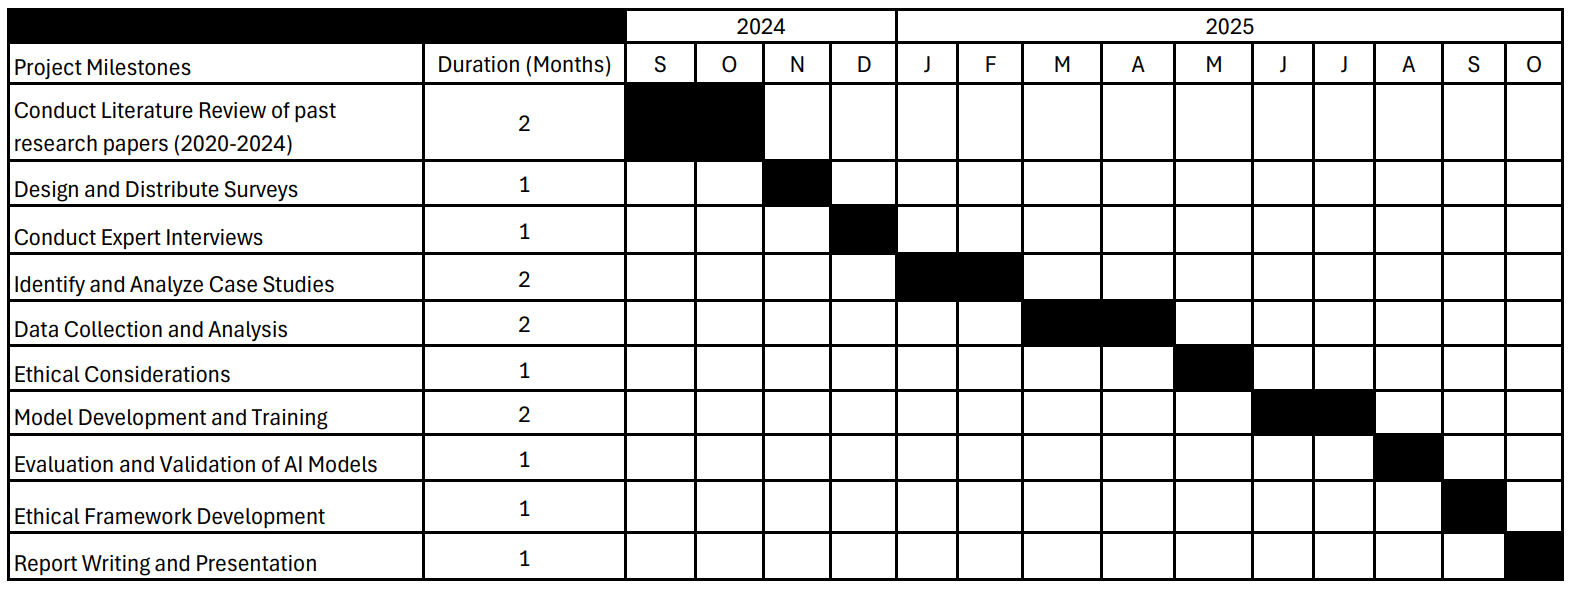
\includegraphics[scale=0.48]{GanttChart Research Milestones.png}\\
\small Figure 6: Research Milestones Gantt Chart \normalsize
\end{center}

Figure 6 above shows a Gantt chart outlining the timeline for our research project on ethical challenges in AI-driven healthcare. The project spans 14 months, from September 2024 to October 2025. It begins with a two-month literature review in September and October 2024, which will establish a solid foundation for the research. In November and December 2024, the team will design and distribute surveys, as well as conduct expert interviews, to gather data from stakeholders. In January to February 2025, the focus shifts to identifying and analyzing relevant case studies for practical insights. Data collection and analysis will take place from March to April 2025, synthesizing both quantitative and qualitative data to provide a comprehensive understanding of the research findings. Ethical considerations are addressed throughout in May 2025. Model development and training occupies June and July 2025, applying AI techniques to develop relevant models. August 2025 is dedicated to evaluation and validation of these models. In September 2025, an ethical framework is developed to guide responsible AI implementation. The project then concludes with report writing and presentation in October 2025, where findings are compiled and shared with stakeholders.

\pagebreak
% ______________________________________________
%           EXPECTED RESULTS AND IMPACT
% ______________________________________________

\section{Expected Results and Impact}
This research will likely provide several important data about the ethical issues involved in AI-driven healthcare, particularly in the context of intelligent health information systems. The latest improvements include:\\

\textbf{7.1 \hspace{5mm} New Insights on AI-Driven Ethical Frameworks}\\
This study will provide an in-depth analysis of the differences between ethical AI principles and their practical application in the healthcare industry. Through a detailed analysis of ethical issues such as algorithmic bias, data privacy, and transparency, the research will highlight how important it is to apply AI ethics across the whole AI life cycle. This framework will enable healthcare organizations and AI developers to build ethically responsible AI systems for medical applications, which will bring on several benefits.\\

\textbf{7.2 \hspace{5mm} Improvement in AI Performance in Retinal Disease Diagnosis}\\
The study will investigate how artificial intelligence can be used to diagnose retinal diseases while offering ethical and technical points of view. By examining AI's capacity to diagnose diseases like age-related macular degeneration and diabetic retinopathy, the study is predicted to show improvements in diagnostic accuracy, early detection, and overall patient outcomes. This investigation will contribute to the growing body of knowledge about the application of AI in particular medical fields where accuracy is crucial for patient care.\\

\textbf{7.3 \hspace{5mm} Bridging the Gap between AI Ethics and Practice}\\
Finding the barriers to applying AI ethics principles in real-world healthcare settings will be an important result. The purpose of this study is to provide useful guidelines and legal frameworks that link theoretical ethical concepts to real-world application in healthcare systems. Including AI technologies with transparency, accountability, and patient-centered care requires commitment to these guidelines.\\

The expected result of this study will lead to important progress in understanding the ethical dilemmas presented by AI-powered healthcare, especially in the field of intelligent health information systems. A new element will be the creation of a thorough framework that bridges the divide between AI ethics principles and their implementation in healthcare. This model will address important ethical issues like bias in algorithms, privacy of data, and transparency, and will provide practical ways to incorporate ethics in all stages of AI development. Furthermore, the research will provide valuable information on how well AI performs in diagnosing retinal diseases, particularly in cases such as diabetic retinopathy and age-related macular degeneration.\\

This assessment will show how AI can improve diagnostic accuracy, enhance early detection, and result in improved patient outcomes. Moreover, this study will offer practical recommendations for closing the divide between ethical values and practical use, presenting a structure for governance that guarantees transparency, accountability, and patient-focused care when implementing AI in clinical environments.\\

This research will have a significant effect on various areas. In terms of society, utilizing AI technologies responsibly with ethical guidelines will enhance trust in AI-based healthcare, tackling issues like bias and data privacy. This will help ensure AI is used fairly in medical decision-making, aiding disadvantaged communities and improving healthcare systems' fairness and transparency. On a national level, the results will assist policymakers and healthcare regulators in creating plans for the ethical incorporation of AI in medical facilities. Through offering guidance on implementing AI responsibly, the study will impact national laws and establish the country as a pioneer in ethical AI advancement.\\

From an economic perspective, the research will showcase how AI has the ability to make healthcare services more efficient, leading to savings in labor expenses and a decreased reliance on invasive treatments, ultimately resulting in more affordable healthcare delivery. Through enhancing effectiveness and facilitating earlier identification of diseases, the proper utilization of AI technologies will decrease the long-term financial strain on healthcare systems, while also opening possibilities for advancement and expansion in the AI healthcare sector.\\

Therefore, it is anticipated that the outcomes of this study will have wide-ranging effects on society, the country, and the economy, aiding in the ethical and influential incorporation of AI in the healthcare field.

\section{Expected Output}
\begin{table}[h]
    \centering
    \begin{adjustbox}{max width=\textwidth}
    \begin{tabular}{|>{\centering\arraybackslash}m{3.5cm}|>{\centering\arraybackslash}m{3.5cm}|>{\centering\arraybackslash}m{2.5cm}|>{\centering\arraybackslash}m{2.5cm}|>{\centering\arraybackslash}m{2.5cm}|>{\centering\arraybackslash}m{2.5cm}|}
        \hline
        \textbf{Disease} & \textbf{Model} & \textbf{Accuracy (\%)} & \textbf{Sensitivity (\%)} & \textbf{Specificity (\%)} & \textbf{AUC-ROC} \\
        \hline
        \multirow{3}{*}{Diabetic Retinopathy} & Traditional & 85 & 82 & 84 & 0.88 \\
         & CNNs (2020) & 87 & 85 & 88 & 0.91 \\
         & CNNs (2022) & 92 & 90 & 92 & 0.95 \\
        \hline
        \multirow{3}{*}{Retinal Detachment} & Traditional & 82 & 80 & 83 & 0.86 \\
         & CNNs (2020) & 85 & 83 & 86 & 0.89 \\
         & CNNs (2022) & 93 & 91 & 93 & 0.96 \\
        \hline
        \multirow{3}{*}{Glaucoma} & Traditional & 80 & 78 & 81 & 0.84 \\
         & CNNs (2020) & 83 & 81 & 84 & 0.88 \\
         & CNNs (2022) & 90 & 88 & 90 & 0.93 \\
        \hline
        \multirow{3}{*}{Retinitis Pigmentosa} & Traditional & 78 & 76 & 79 & 0.82 \\
         & CNNs (2020) & 81 & 79 & 82 & 0.85 \\
         & CNNs (2022) & 89 & 87 & 89 & 0.92 \\
        \hline
        \multirow{2}{*}{All Diseases (2022)} & Machine Learning & 88 & 86 & 89 & 0.91 \\
         & AI-Assisted Interfaces & 87 & 85 & 88 & 0.90 \\
        \hline
    \end{tabular}
    \end{adjustbox}
\end{table}
\begin{center}
\small Table 1: Performance Metrics of AI Models for Retinal Diseases\normalsize
\end{center}

As for the output of our research, the table above compares various AI models, including Convolutional Neural Networks (CNNs), machine learning algorithms, and AI-assisted conversational interfaces, in diagnosing retinal diseases from 2020 to 2022. Performance metrics such as accuracy, sensitivity, specificity, and the Area Under the Receiver Operating Characteristic Curve (AUC-ROC) are listed for each model.

For Diabetic Retinopathy, the accuracy of CNNs would improve from 87\% in 2020 to 92\% in 2022, with corresponding increases in sensitivity (from 85\% to 90\%), specificity (from 88\% to 92\%), and AUC-ROC (from 0.91 to 0.95). Similar trends would be observed for Retinal Detachment, Glaucoma, and Retinitis Pigmentosa, indicating significant enhancements in all performance metrics. By 2022, machine learning algorithms and AI-assisted interfaces would also demonstrate high performance, showcasing the robustness of various AI technologies.

This data indicates the significant improvements in AI model performance for retinal disease detection and diagnosis over the years, showcasing AI's potential to improve healthcare outcomes.
\pagebreak

% ______________________________________________
%                    REFERENCES
% ______________________________________________
\nocite{Georgieva2022}
\nocite{Hassani2023}

%References
\bibliographystyle{apacite}
\bibliography{MyBib}{}   

\end{document}